Após a documentação dos requisitos funcionais e não funcionais sob a forma de casos de uso, foi possível obter um melhor entendimento do que deveria ser desenvolvido. Com a conclusão desta etapa, partiu-se para a elaboração do modelo conceitual, visando representar, em alto nível, as abstrações efetuadas e as associações entre elas. O modelo conceitual resultante é ilustrado na Figura \ref{fig:modeloConceitual}.

\begin{figure}[H]
	\centering
	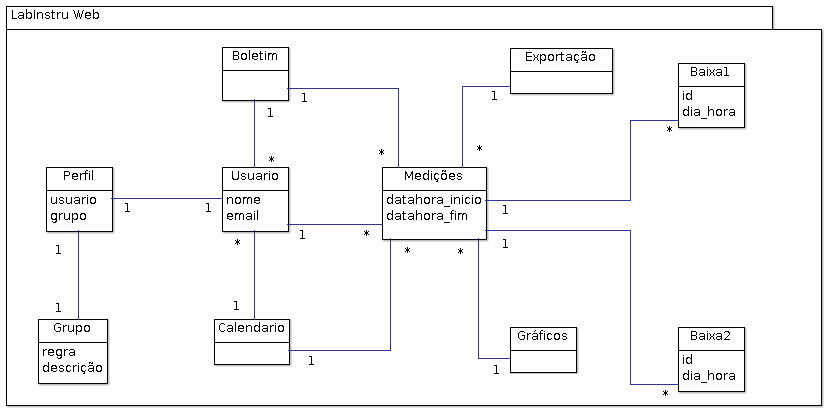
\includegraphics[scale=0.8]{img/ModeloConceitual.png}
	\caption{Módelo Conceitual - LabInstru Web.}
	\label{fig:modeloConceitual}
\end{figure}

Neste modelo, a entidade \texttt{Usuário} representa os atores que irão interagir com a aplicação. Cada usuário é encapsulado em um \texttt{Perfil} e os perfis são organizados em um \texttt{Grupo}, que contém um conjunto de regras e descrições. Há dois perfis de usuários: \texttt{Admin}, que possui os privilégios especiais de cadastrar novas medições provenientes da estação meteorológica da EST e manter os usuários; e \texttt{User}, grupo elementar, que utiliza as funcionaldiades disponibilizadas pela aplicação, tais como consulta às medições, exportação de dados, geração de boletins meteorológicos, dentre outras. É interessante notar que, embora não ressaltado neste modelo, todo \texttt{Admin} é um \texttt{User}.

Em relação aos dados meteorológicos da aplicação, estes são organizados em \texttt{Medições}, que podem conter dados oriundos do \texttt{Baixa1} ou \texttt{Baixa2}, advindos de dois tipos de arquivos distintos da estação meteorológica da EST. Em virtude deste ser um modelo de alto-nível, os atributos particulares que diferenciam e caracterizam o \texttt{Baixa1} e o \texttt{Baixa2} não estão detalhados.

Com entidadas do tipo \texttt{Medição}, os usuários podem então gerar um boletim meteorológico (\texttt{Boletim}), visualizar o calendário de disponibilidade (\texttt{Calendario}), gerar gráficos (\texttt{Gráficos}) ou exportar os dados produzidos (\texttt{Exportação}).

As ideias fundamentais contidas neste modelo conceitual serviram como ponto de partida para a elaboração dos elementos posteriores, detalhados nas seções a seguir.
